% Document Class
%________________________________________________________________________
\documentclass[12pt]{report}
%________________________________________________________________________

% Imported Packages
%________________________________________________________________________
\usepackage{alltt}
\usepackage{amsmath}
\usepackage{amssymb}
\usepackage{amstext}
\usepackage{amsthm}
\usepackage{bytefield}
\usepackage{color}
\usepackage{Styles/eclbip}
\usepackage{enumerate}
\usepackage{epic}
\usepackage{Styles/fancyheadings}
\usepackage[hmargin=20mm,vmargin=30mm]{geometry}
\usepackage{graphicx}
\usepackage[pdfpagelabels,hypertexnames=false,breaklinks=true,
			bookmarksopen=true,bookmarksopenlevel=2]{hyperref}
\usepackage{ifthen}
\usepackage{listings}
\usepackage{makeidx}
\usepackage{Styles/natbib}
\usepackage{Styles/setspace}
\usepackage{subcaption}
\usepackage{Styles/thesis}
\usepackage{xcolor}
\usepackage{xspace}
\usepackage[all]{xy}
\usepackage{textgreek}
\usepackage{lmodern}
\usepackage{parskip}
\usepackage{comment}
\usepackage{Styles/agda}
\usepackage{Styles/AgdaChars}
\usepackage{Styles/edcomms}

%________________________________________________________________________

% Macros and Commands
%________________________________________________________________________

% Include the macro files
%________________________________________________________________________
%_________________     BEGIN LINEAR NOTATION MACROS    __________________
%________________________________________________________________________

% Linear Notation: Standard
\newcommand{\lnotation}[4]{
	\def\third:{#3} 
	\def\possiblyone:{} 
	\def\possiblytwo:{~}
	\def\possiblythree:{ }
	\def\divide{\;#1\hspace*{-0pt}( #2\; \mid: \; #4 \, )}
	\def\nodivide{\;#1\hspace*{-0pt}( #2\;\mid\; #3\;:\;#4 \, )}
	\ifx\third\possiblyone\divide
		\else\ifx\third\possiblytwo\divide
		\else \ifx\third\possiblythree\divide
		\else \nodivide\fi\fi\fi}

% Linear Notation: Standard (Big Parentheses)
\newcommand{\biglnotation}[4]{
	\def\third:{#3} 
	\def\possiblyone:{} 
	\def\possiblytwo:{~}
	\def\possiblythree:{ }
	\def\divide{\;#1\hspace*{-0pt}\big( #2\; \mid: \; #4 \, \big)}
	\def\nodivide{\;#1\hspace*{-0pt}\big( #2\;\mid\; #3\;:\;#4 \, \big)}
	\ifx\third\possiblyone\divide
		\else\ifx\third\possiblytwo\divide
		\else \ifx\third\possiblythree\divide
		\else \nodivide\fi\fi\fi}

% Linear Notation: Standard (Extra Big Parentheses)
\newcommand{\bigglnotation}[4]{
	\def\third:{#3} 
	\def\possiblyone:{} 
	\def\possiblytwo:{~}
	\def\possiblythree:{ }
	\def\divide{\;#1\hspace*{-0pt}\bigg( #2\; \mid: \; #4 \, \bigg)}
	\def\nodivide{\;#1\hspace*{-0pt}\bigg( #2\;\mid\; #3\;:\;#4 \, \bigg)}
	\ifx\third\possiblyone\divide
		\else\ifx\third\possiblytwo\divide
		\else \ifx\third\possiblythree\divide
		\else \nodivide\fi\fi\fi}
 
% Linear Notation: Standard (No Ending Parentheses)
\newcommand{\wplnotation}[4]{
	\def\third:{#3} 
	\def\possiblyone:{} 
	\def\possiblytwo:{~}
	\def\possiblythree:{ }
	\def\divide{\;#1\hspace*{-0pt}\bigg( #2\; \mid: \; #4 \, }
	\def\nodivide{\;#1\hspace*{-0pt}\bigg( #2\;\mid\; #3\;:\;#4 \, }
	\ifx\third\possiblyone\divide
		\else\ifx\third\possiblytwo\divide
		\else \ifx\third\possiblythree\divide
		\else \nodivide\fi\fi\fi}

% Linear Notation: David Gries
\newcommand{\grieslnotation}[4]{
	\def\third:{#3} 
	\def\possiblyone:{} 
	\def\possiblytwo:{~}
	\def\possiblythree:{ }
	\def\divide{(#1 #2\; \mid : \; #4 \, )}
	\def\nodivide{(#1 #2\;\mid\; #3\;:\;#4 \, )}
	\ifx\third\possiblyone\divide
		\else\ifx\third\possiblytwo\divide
		\else \ifx\third\possiblythree\divide
		\else \nodivide\fi\fi\fi}

%________________________________________________________________________
%_________________      END LINEAR NOTATION MACROS     __________________
%________________________________________________________________________

%________________________________________________________________________
%_________________       BEGIN SET NOTATION MACROS     __________________
%________________________________________________________________________

% Set Notation: David Gries
\newcommand{\griesset}[3]{
	\def\second:{#2} 
	\def\possiblyone:{} 
	\def\possiblytwo:{~}
	\def\possiblythree:{ }
	\def\divide{\{#1\; \mid : \; #3 \, \}}
	\def\nodivide{\{#1\;\mid\; #2\;:\;#3 \, \}}
	\ifx\second\possiblyone\domvide
		\else \ifx\second\possiblytwo\divide
		\else \ifx\second\possiblythree\divide
		\else \nodivide\fi\fi\fi}

% Set Notation: Standard Enumeration
\newcommand{\set}[1]{\{#1\}}

% Set Notation: Standard Comprehension
\newcommand{\sets}[2]{\{#1\; \mid \; #2\}}

% Set Notation: Standard (Big Parentheses)
\newcommand{\bigset}[2]{\big\{#1\; \mid \; #2\big\}}

% Set Notation: Standard (Extra Big Parentheses)
\newcommand{\biggset}[2]{\bigg\{#1\; \mid \; #2\bigg\}}

%________________________________________________________________________
%_________________        END SET NOTATION MACROS      __________________
%________________________________________________________________________

%________________________________________________________________________
%_________________        BEGIN STRUCTURE MACROS       __________________
%________________________________________________________________________

% Common Calligraphic Names
\newcommand{\C}{{\cal{C}}}
\newcommand{\F}{{\cal{F}}}
\newcommand{\II}{{\cal{I}}}
\newcommand{\M}{{\cal{M}}}
\newcommand{\N}{{\cal{N}}}
\newcommand{\R}{{\cal{R}}}
\newcommand{\Rel}{{\cal{R}}el}
\newcommand{\T}{{\cal{T}}}
\newcommand{\Z}{{\cal{Z}}}
\newcommand{\one}[1]{1_{#1}}

% Semi-Group
\newcommand{\semigroup}[2]{\big(#1, #2 \big)}

% Monoid
\newcommand{\monoid}[3]{\big(#1, #2, #3 \big)}

% Semi-Rings
\newcommand{\nsemiring}[3]{\big(#1, #2, #3\big)}
\newcommand{\semirng}[4]{\big(#1, #2, #3, #4\big)}
\newcommand{\semiring}[5]{\big(#1, #2, #3, #4, #5\big)}

% Group
\newcommand{\group}[4]{\big(#1, #2, #3, #4\big)}

% Semi-Module
\newcommand{\semimodule}[3]{\big(_{#1}#2, #3\big)}

% Relational Lattice
\newcommand{\latticeRel}[2]{\big(#1, #2 \big)}

% Algebraic Lattice
\newcommand{\latticeAlg}[3]{\big(#1, #2,  #3\big)}

%________________________________________________________________________
%_________________         END STRUCTURE MACROS        __________________
%________________________________________________________________________

%________________________________________________________________________
%_________________    BEGIN PROOF ENVIRONMENT MACROS   __________________
%________________________________________________________________________

% Spacing
\newlength{\interligne}

% Begin and End Basic Proof Enviroment
\newcommand{\Beginproof}{\dimen123=\linewidth \dimen124=\linewidth
	\advance\dimen123 by -25mm \advance\dimen124 by -5mm
	\advance\dimen123 by -\parindent \advance\dimen124 by -\parindent
	\setlength{\interligne}{\baselineskip}
	\setlength{\baselineskip}{1.2\baselineskip}
    	\begin{tabbing}
    		\hspace*{\parindent}\= \hspace*{5mm}\= \kill \+ \kill}
			\newcommand {\Endproof}
		{\end{tabbing}
    \setlength{\baselineskip}{\interligne}}

% Comment
\newcommand{\com}[1]{\> \hspace*{15mm}
	$\langle$~\parbox[t]{\dimen123}{ #1 $\rangle$}\\}

% Coloured Comment
\newcommand{\comc}[1]{\> \hspace*{15mm}
	$\langle$~\parbox[t]{\dimen123}{ \textcolor{red}{#1} $\rangle$}\\}

% Predicate
\newcommand{\pred}[1]{\>\parbox[t]{\dimen124}{#1}\\}

% Comment Separator
\newcommand{\hsep}{\quad\&\quad}


% Begin and End Itemized/Enumerated Proof Enviroment
% Use \Beginproofitem when a proof begins the text of an \item 
% and when we want the proof to be indented.
\newcommand{\Beginproofitem}{\dimen123=\linewidth \dimen124=\linewidth
	\advance\dimen123 by -20mm \advance\dimen124 by -5mm
	\advance\dimen124 by -\parindent
    	\begin{tabbing}
    		\hspace*{5mm}\= \kill}
			\newcommand {\Endproofitem}
	{\end{tabbing}}

% Tabbing
% Gives the same indentation as \Beginproof and \dspec, 
% but there is no predefined tabs
\newcommand {\Begingtabin}{
	\begin{tabbing}
    	\hspace*{\parindent}\= \kill \+ \kill}
		\newcommand {\Endtabin}
	{\end{tabbing}}

% Begin and End Basic Program Specification Enviroment
\newcommand{\Begingspec}{
	\begin{tabbing}
    	\hspace*{\parindent}\= \hspace*{5mm}\=\hspace*{5mm}\=\hspace*{5mm}\=
			\hspace*{5mm}\=\hspace*{5mm} \kill \+ \kill}
		\newcommand {\Endspec}
	{\end{tabbing}}

% Begin and End Itemized/Enumerated Program Specification Enviroment
% Use \Beginproofitem when a proof begins the text of an \item 
% and when we do not want that the specification be indented
\newcommand {\Beginspecitem}{
	\begin{tabbing}
    	\hspace*{5mm}\=\hspace*{5mm}\=\hspace*{5mm}\=
    	\hspace*{5mm}\=\hspace*{5mm} \kill}
		\newcommand {\Endspecitem}
	{\end{tabbing}}

% Multiline Proof Formulas
\newcommand{\nln}{@{}l@{}}
\newenvironment{displaymany}{\[ \begin{array}{\nln}}{\end{array} \]}

%________________________________________________________________________
%_________________     END PROOF ENVIRONMENT MACROS    __________________
%________________________________________________________________________

%________________________________________________________________________
%_________________         BEGIN EQUATION MACROS       __________________
%________________________________________________________________________

% When ShowEqSourceStructure is at 1, it shows the argument of \eqfrom
\newcommand{\ShowEqSourceStructure}{1}

\newcommand{\eqname}[1]{\textcolor{black}{\mbox{#1}}}

\newcommand{\eqfrom}[1]{
	\ifthenelse{\ShowEqSourceStructure=1}
	{ \quad {\textcolor{red}{\mbox{#1}}}} {\quad} }

%________________________________________________________________________
%_________________          END EQUATION MACROS        __________________
%________________________________________________________________________

%________________________________________________________________________
%_________________          BEGIN LOGIC MACROS         __________________
%________________________________________________________________________

% Logical Connectives: Constants
\newcommand{\true}{\textsf{true}}
\newcommand{\false}{\textsf{false}}

% Logical Connectives: Unary
\renewcommand{\Not}{\neg}

% Logical Connectives: Binary	 
%\newcommand{\Or}{\mathrel{\vee}}
\newcommand{\Ors}{\;\Or\;}
\newcommand{\AAnd}{\mathrel{\wedge}}
\newcommand{\nAnd}{\;\AAnd\;}
\newcommand{\Imp}{\mathrel{\rightarrow}}
\newcommand{\Impl}{\mathrel{\leftarrow}}
\newcommand{\Iff}{\mathrel{\leftrightarrow}}
\newcommand{\mOr}{\textrm{\ or\ }}  
\newcommand{\mAnd}{\textrm{\ and\ }} 
\newcommand{\mImp}{\;\Longrightarrow\;}  
\newcommand{\mImpl}{\;\Longleftarrow\;}  
\newcommand{\mIff}{\;\Longleftrightarrow\;} 
\newcommand{\dIff}{\mathrel{\stackrel{\scriptscriptstyle
	\mbox{\tiny{\texsf{def}}}}{\Iff}}}

%________________________________________________________________________
%_________________           END LOGIC MACROS          __________________
%________________________________________________________________________

%________________________________________________________________________
%_________________           BEGIN SET MACROS          __________________
%________________________________________________________________________

% Common Sets
\newcommand{\ONE}{1\!\!1}
\newcommand{\Prime}{\mathbb{P}}
\newcommand{\Bool}{\mathbb{B}}
\newcommand{\Nat}{\mathbb{N}}
\newcommand{\Real}{\mathbb{R}}
\newcommand{\Integer}{\mathbb{Z}}
\newcommand{\STtop}{\textsf{U}}
\newcommand{\STbot}{\emptyset}
\newcommand{\STpowerset}[1]{{\cal{P}}(#1)}

% Operators: Unary
\newcommand{\STcomplement}[1]{\overline{#1}}
\newcommand{\STcplOP}{\overline{\phantom{Y}\,}}

% Operators: Binary
\newcommand{\STleq}{\subseteq}
\newcommand{\STlt}{\subset}
\newcommand{\STgeq}{\supseteq}
\newcommand{\STgt}{\supset}
\newcommand{\STjoin}{\; \cup \;}
\newcommand{\STmeet}{\; \cap \;}

% Closures
\newcommand{\rtclosure}[1]{#1^*{}}	
\newcommand{\rtc}{\rtclosure}
\newcommand{\tclosure}[1]{#1^+{}}	
\newcommand{\tcl}{\tclosure}

%________________________________________________________________________
%_________________            END SET MACROS           __________________
%________________________________________________________________________

%________________________________________________________________________
%_________________    BEGIN REALTION ALGEBRA MACROS    __________________
%________________________________________________________________________

% Common Relations
\newcommand{\RAtop}{\mathbb{L}}
\newcommand{\RAid}{\mathbb{I}}
\newcommand{\RAdi}{\RAcomplement{\RAid}}
\newcommand{\RAbot}{\emptyset}

% Operators: Unary
\newcommand{\RAcomplement}[1]{\overline{#1}}
\newcommand{\RAcplOP}{\overline{\phantom{Y}\,}}
\newcommand{\internalconverse}[1]{#1^{\mkern-1mu{}{\raise0.1ex\hbox{\tiny$\smallsmile\,$}}}\kern-0.1em{}}
\newcommand{\RAconverse}[1]{\internalconverse{#1}}
\newcommand{\RAconverseOP}{\RAconverse{}\,}

% Operators: Binary
\newcommand{\RAcomp}{\mathop{\kern-.5pt\raise.3ex\hbox{\footnotesize\rm;}}}
\newcommand{\RAleq}{\sqsubseteq}
\newcommand{\RAgeq}{\sqsupseteq}
\newcommand{\RAjoin}{\; \sqcup \;}
\newcommand{\RAmeet}{\; \sqcap \;}
\newcommand{\RAcompose}[2]{#1\,\mbox{$\RAcomp$}\, #2}
\newcommand{\RAcomposet}[3]{\RAcompose{\RAcompose{#1}{#2}} {#3}}
\newcommand{\RAcomposeq}[4]{\RAcompose{\RAcompose{#1}{#2}} {\RAcompose {#3}{#4}}}
\newcommand{\RAcomposec}[5]{\RAcompose{\RAcomposeq{#1}{#2}{#3}{#4}} {#5}}
\newcommand{\RAcomposes}[6]{\RAcompose{\RAcomposet{#1}{#2}{#3}} {\RAcomposet {#4}{#5} {#6}}}
\newcommand{\rressymbol}{\backslash}
\newcommand{\RArightresidual}[2]{{#1}\rressymbol{#2}}
\newcommand{\lressymbol}{/}
\newcommand{\RAleftresidual}[2]{{#1}\lressymbol{#2}}
\newcommand{\RAsyq}[2]{\textsf{syq}(#1,#2)}

% Others
\newcommand{\RAsubset}{\sqsubset}
\newcommand{\elmtspecial}{\sharp}

% Types
\newcommand{\typerel}[2]{#1 \leftrightarrow #2}
\newenvironment{arra}[2][]{\begin{array}[#1]{@{}#2@{}}}{\end{array}} 
\newenvironment{tabul}[2][]{\begin{tabular}[#1]{@{}#2@{}}}{\end{tabular}} 

%________________________________________________________________________
%_________________     END REALTION ALGEBRA MACROS     __________________
%________________________________________________________________________

%________________________________________________________________________
%_________________       BEGIN HOARE LOGIC MACROS      __________________
%________________________________________________________________________

% Guards
\newcommand{\guardsymb}{\lceil\!\:\!\!\rfloor}
\newcommand{\guardif}[2]{\ifs \quad #1 \longrightarrow #2}
\newcommand{\guardb}[2]{\guardsymb\; \quad #1 \longrightarrow #2}
\newcommand{\guarde}{\fis}

% Keywords
\newcommand{\gives}{\longrightarrow}
\newcommand{\derive}[2]{\overset{#2}{\underset{#1}{\longrightarrow}}}
\newcommand{\gderive}[1]{\overset{#1}{\underset{G}{\longrightarrow}}}
\newcommand{\nocc}[2]{\neg\occurs('#1',\; '#2')}
\newcommand{\odd}[1]{\oddd(#1)}
\newcommand{\even}[1]{\evenn(#1)}
\newcommand{\hoare}[3]{\{#1\}\;#2\;\{#3\}}
\newcommand{\lpthoare}[4]{
	\begin{tabbing}
 		$\{#1\}\;\mbox{\bp{$#2$}}\;$\=$\{#3$\\
        \> $\;\;#4\;\}$
	\end{tabbing}
}
\newcommand{\choare}[3]{\mbox{\bp{$\{#1\}$}}\;#2\;\mbox{\mpoint{$\{#3\}$}}}
\newcommand{\massign}[2]{\mbox{$#1\;:=\;#2$} }
\newcommand{\subst}[2]{\left[\mbox{$#1\;:=\;#2$}\right] }

%________________________________________________________________________
%_________________        END HOARE LOGIC MACROS       __________________
%________________________________________________________________________

%________________________________________________________________________
%_________________      BEGIN COMMON SYMBOL MACROS     __________________
%________________________________________________________________________

% Functions / Relations
\newcommand{\dom}[1]{\textsf{dom\ }\!(#1)}	
\newcommand{\ran}[1]{\textsf{ran\ }\!(#1)}	
\newcommand{\tuple}[1]{(#1)}		

% Sets
\newcommand{\abs}[1]{|#1|}
\newcommand{\length}[1]{|#1|}
\newcommand{\card}[1]{\# \! #1}
\newcommand{\sizeset}[1]{\mid  \! #1 \! \mid}
\newcommand{\cardp}[1]{\# \!\left(#1\right)}

% Vectors
\newcommand{\zero}{\hat{0}}
\newcommand{\un}{\hat{1}}
\newcommand{\lator}{\;\mbox{\scalebox{0.5}{$\nabla$}}\;}
\newcommand{\latand}{\; \mbox{\scalebox{0.5}{$\triangle$}}\;}

% Prime
\newcommand{\p}[1]{\mbox{$#1'$}}

% Definitions
\newcommand{\deq}{\spaces{\stackrel{\textrm{def}}{=}}}
\newcommand{\defiff}{\spaces{\stackrel{\textrm{def}}{\mIff}}}

% Equivalences
\newcommand{\sequiv}[2]{#1\approx #2}
\newcommand{\equivwrt}[3]{#1\approx_{#2} #3}
\newcommand{\class}[1]{\left[#1\right]}

%________________________________________________________________________
%_________________       END COMMON SYMBOL MACROS      __________________
%________________________________________________________________________

%________________________________________________________________________
%_________________         BEGIN KEYWORD MACROS        __________________
%________________________________________________________________________

% Fonts and Colours
\newcommand{\keyw}[1]{{\textsf{#1}}}
\newcommand{\ckeyw}[1]{\mbox{\textcolor{blue}{\textsf{#1}}}}

% Spacing
\newcommand{\rspace}[1]{#1\ }
\newcommand{\lspace}[1]{\ #1}
\newcommand{\spaces}[1]{\,#1\,}

% Keywords
\newcommand{\oddd}{\keyw{odd}}
\newcommand{\evenn}{\keyw{even}}
\newcommand{\occurs}{\keyw{occurs}}
\newcommand{\aborts}{\keyw{abort}}
\newcommand{\begins}{\rspace{\keyw{begin}}}
%\newcommand{\ends}{\lspace{\keyw{end}}}
\newcommand{\divs}{\spaces{\keyw{div}}}
\newcommand{\dos}{\spaces{\keyw{do}}}
\newcommand{\elses}{\spaces{\keyw{else}}}
\newcommand{\skips}{\spaces{\keyw{skip}}}
\newcommand{\error}{\keyw{error}}
\newcommand{\fis}{\lspace{\keyw{fi}}}
\newcommand{\fors}{\spaces{\keyw{for}}}
\newcommand{\ifs}{\rspace{\keyw{if}}}
\newcommand{\mods}{\spaces{\keyw{mod}}}
\newcommand{\notts}{\rspace{\keyw{not}}}
\newcommand{\ods}{\lspace{\keyw{od}}}
\newcommand{\procs}{\rspace{\keyw{proc}}}
\newcommand{\thens}{\spaces{\keyw{then}}}
\newcommand{\vars}{\rspace{\keyw{var}}}
\newcommand{\whiles}{\rspace{\keyw{while}}}
\newcommand{\wrts}{\spaces{\keyw{wrt}}}
\newcommand{\revs}{\spaces{\keyw{rev}}}

% Coloured Keywords
\newcommand{\coddd}{\ckeyw{odd}}
\newcommand{\cevenn}{\ckeyw{even}}
\newcommand{\coccurs}{\ckeyw{occurs}}
\newcommand{\caborts}{\ckeyw{abort}}
\newcommand{\cbegins}{\rspace{\ckeyw{begin}}}
\newcommand{\cends}{\lspace{\ckeyw{end}}}
\newcommand{\cdivs}{\spaces{\ckeyw{div}}}
\newcommand{\cdos}{\spaces{\ckeyw{do}}}
\newcommand{\celses}{\spaces{\ckeyw{else}}}
\newcommand{\cskips}{\spaces{\ckeyw{skip}}}
\newcommand{\cerror}{\ckeyw{error}}
\newcommand{\cfis}{\lspace{\ckeyw{fi}}}
\newcommand{\cfors}{\spaces{\ckeyw{for}}}
\newcommand{\cifs}{\rspace{\ckeyw{if}}}
\newcommand{\cmods}{\spaces{\ckeyw{mod}}}
\newcommand{\cnotts}{\rspace{\ckeyw{not}}}
\newcommand{\cods}{\lspace{\ckeyw{od}}}
\newcommand{\cprocs}{\rspace{\ckeyw{proc}}}
\newcommand{\cthens}{\spaces{\ckeyw{then}}}
\newcommand{\cvars}{\rspace{\ckeyw{var}}}
\newcommand{\cwhiles}{\rspace{\ckeyw{while}}}
\newcommand{\cwrts}{\spaces{\ckeyw{wrt}}}
\newcommand{\crevs}{\spaces{\ckeyw{rev}}}

%________________________________________________________________________
%_________________          END KEYWORD MACROS         __________________
%________________________________________________________________________

%________________________________________________________________________
%_________________     BEGIN COVERT CHANNEL MACROS     __________________
%________________________________________________________________________

% Sets
\newcommand\Data{\mathbb{D}}

% Agents
\newcommand{\AgentOne}{\textrm{agent $A$}\@\xspace}
\newcommand{\AgentTwo}{\textrm{agent $B$}\@\xspace}
\newcommand{\Monitor}{\textrm{$M$}\@\xspace}

% Information
\newcommand{\CInfo}{\Phi_C}
\newcommand{\OInfo}{\Phi_O}

% Operations: Combining Information
\newcommand{\opA}{\odot}
\newcommand{\opB}{\otimes}
\newcommand{\opC}{\oplus}

% Relview Type Text
\newcommand{\relview}{\texttt{RELVIEW}}

%________________________________________________________________________
%_________________      END COVERT CHANNEL MACROS      __________________
%________________________________________________________________________

%________________________________________________________________________
%_________________       BEGIN HIGLIGHTING MACROS      __________________
%________________________________________________________________________

% Highlight Text
\newcommand{\hl}[1]{\colorbox{grey}{#1}}

% Coloured Boxes For ByteField
\newcommand{\colorbitbox}[3]
	{\rlap{\bitbox{#2}{\color{#1}\rule{\width}{\height}}}\bitbox{#2}{#3}}
\newcommand{\colorwordbox}[3]
	{\rlap{\wordbox{#2}{\color{#1}\rule{\width}{\height}}}\wordbox{#2}{#3}}

%________________________________________________________________________
%_________________        END HIGLIGHTING MACROS       __________________
%________________________________________________________________________



%________________________________________________________________________
%_________________       BEGIN ABBREVIATION MACROS     __________________
%________________________________________________________________________

% These macros require the inclusion of the xspace package 
% \usepackage{xspace}

% Example
\newcommand{\eg}{\textrm{e.g.,}\@\xspace}

% That Is To Say
\newcommand{\ie}{\textrm{i.e.,}\@\xspace}

% And So On
\newcommand{\etc}{\textrm{etc.}\@\xspace}

% And Others
\newcommand{\etal}{\textrm{et al.}\@\xspace}

% With Respect To
\newcommand{\wrt}{\textrm{w.r.t.}\@\xspace}

% Vice Versa
\newcommand{\vrsa}{\textrm{vice versa}\@\xspace}

%________________________________________________________________________
%_________________        END ABBREVIATION MACROS      __________________
%________________________________________________________________________



%________________________________________________________________________
%_________________          BEGIN REVIEW MACROS        __________________
%________________________________________________________________________

% These macros require the inclusion of the color and ulem package 
% \usepackage{color}
% \usepackage{ulem}

% Color Definitions
\definecolor{darkred}{rgb}{0.75,0.0,0.0}
\definecolor{darkgreen}{rgb}{0.0,0.6,0.0}
\definecolor{darkblue}{rgb}{0.0,0.0,0.6}
\definecolor{darkcyan}{rgb}{0.0,0.6,0.6}
\definecolor{darkmagenta}{rgb}{0.6,0.0,0.6}
\definecolor{darkyellow}{rgb}{0.6,0.6,0.0}
\definecolor{lightred}{rgb}{1.0,0.9,0.9}
\definecolor{lightgreen}{rgb}{0.9,1.0,0.9}
\definecolor{lightblue}{rgb}{0.9,0.9,1.0}
\definecolor{lightcyan}{rgb}{0.8,1.0,1.0}
\definecolor{lightmagenta}{rgb}{1.0,0.8,1.0}
\definecolor{lightyellow}{rgb}{1.0,1.0,0.8}
\definecolor{paleyellow}{rgb}{1.0,1.0,0.8}
\definecolor{amber}{rgb}{1.0,0.8,0.0}
\definecolor{darkamber}{rgb}{1.0,0.5,0.0}
\definecolor{webgreen}{rgb}{0,0.5,0}
\definecolor{webbrown}{rgb}{0.6,0,0}
\definecolor{grey}{rgb}{0.65,0.65,0.65}

% Notes
\newcommand{\mynote}[2]{
	\ifthenelse{\equal{#1}{0}}{\textcolor{darkamber}{#2}}{}
  	\ifthenelse{\equal{#1}{1}}{\textcolor{darkmagenta}{#2}}{}
  	\ifthenelse{\equal{#1}{2}}{\textcolor{blue}{#2}}{}
  	\ifthenelse{\equal{#1}{3}}{\textcolor{green}{#2}}{}
}

\newcommand{\newtxt}[2]{
  	\ifthenelse{\equal{#1}{0}}{\textcolor{darkamber}{#2}}{}
  	\ifthenelse{\equal{#1}{1}}{\textcolor{darkmagenta}{#2}}{}
  	\ifthenelse{\equal{#1}{2}}{\textcolor{blue}{#2}}{}
  	\ifthenelse{\equal{#1}{3}}{\textcolor{green}{#2}}{}
}

\newcommand{\newissue}[2]{
  	\ifthenelse{\equal{#1}{0}}{\textcolor{darkcyan}{#2}}{}
  	\ifthenelse{\equal{#1}{1}}{\textcolor{cyan}{#2}}{}
  	\ifthenelse{\equal{#1}{2}}{\textcolor{blue}{#2}}{}
  	\ifthenelse{\equal{#1}{3}}{\textcolor{green}{#2}}{}
}

\newcommand{\flag}[2]{
  	\ifthenelse{\equal{#1}{0}}{~~~\newline$\circ$\uwave{\textcolor{darkamber}{#2}}}{}
  	\ifthenelse{\equal{#1}{1}}{~~~\newline$\circ$\uwave{\textcolor{darkmagenta}{#2}}}{}
  	\ifthenelse{\equal{#1}{2}}{~~~\newline$\circ$\uwave{\textcolor{blue}{#2}}}{}
  	\ifthenelse{\equal{#1}{3}}{~~~\newline$\circ$\uwave{\textcolor{green}{#2}}}{}
}

\newcommand{\torevisit}[2]{
  	\ifthenelse{\equal{#1}{0}}{\textcolor{darkamber}{\uwave{#2}}}{}
  	\ifthenelse{\equal{#1}{1}}{\textcolor{darkmagenta}{\uwave{#2}}}{}
  	\ifthenelse{\equal{#1}{2}}{\textcolor{blue}{\uwave{#2}}}{}
  	\ifthenelse{\equal{#1}{3}}{\textcolor{green}{\uwave{#2}}}{}
}

\newcommand{\suggest}[2]{
  	\ifthenelse{\equal{#1}{0}}{\textcolor{darkamber}{\uline{Suggestion:} #2}}{}
  	\ifthenelse{\equal{#1}{1}}{\textcolor{darkmagenta}{\uline{Suggestion:} \uline{Suggestion:} #2}}{}
  	\ifthenelse{\equal{#1}{2}}{\textcolor{blue}{\uline{Suggestion:} #2}}{}
  	\ifthenelse{\equal{#1}{3}}{\textcolor{green}{\uline{Suggestion:} #2}}{}
}

\newcommand{\takeout}[2]{
  	\ifthenelse{\equal{#1}{0}}{\textcolor{darkamber}{\sout{#2}}}{}
  	\ifthenelse{\equal{#1}{1}}{\textcolor{darkmagenta}{\sout{#2}}}{}
  	\ifthenelse{\equal{#1}{2}}{\textcolor{blue}{\sout{#2}}}{}
  	\ifthenelse{\equal{#1}{3}}{\textcolor{green}{\sout{#2}}}{}
}

\newcommand{\replace}[3]{
  	\ifthenelse{\equal{#1}{0}}{\textcolor{darkamber}{\sout{#2}} \textcolor{darkamber}{#3}}{}
  	\ifthenelse{\equal{#1}{1}}{\textcolor{darkmagenta}{\sout{#2}} \textcolor{darkmagenta}{#3}}{}
  	\ifthenelse{\equal{#1}{2}}{\textcolor{blue}{\sout{#2}} \textcolor{blue}{#2}}{}
  	\ifthenelse{\equal{#1}{3}}{\textcolor{green}{\sout{#2}} \textcolor{green}{#2}}{}
}

%________________________________________________________________________
%_________________           END REVIEW MACROS         __________________
%________________________________________________________________________

%________________________________________________________________________
%_________________       BEGIN ENVIRONMENT MACROS      __________________
%________________________________________________________________________

% Definition
\newtheorem{definition}{Definition}[section]

% Theorem
\newtheorem{theorem}{Theorem}[section]

% Proposition
\newtheorem{proposition}[theorem]{Proposition}

% Axiom
\newtheorem{axiom}{Axiom}[section]

% Corollary
\newtheorem{corollary}{Corollary}[section]

% Example
\newtheorem{example}{Example}[section]

% Program
\newtheorem{program}{Program}[section]

%________________________________________________________________________
%_________________        END ENVIRONMENT MACROS       __________________
%________________________________________________________________________



%________________________________________________________________________
%_________________           BEGIN INDEX MACROS        __________________
%________________________________________________________________________

% Italicized Page Number (For Definitions)
% e.g. \index{test|ital} = test, \emph{3}
\newcommand{\ital}[1]{{\it #1}} 

% Page Spans
% e.g. \index{test|nn} = test, 4n
\newcommand{\numspan}[1]{#1n}

% Italicize in Text and Index
\newcommand{\itindex}[1]{\emph{#1}\index{#1}}

%________________________________________________________________________
%_________________            END INDEX MACROS         __________________
%________________________________________________________________________




% Import the General Thesis Information
% Write your thesis title
\title{(Re-)Creating sharing in Agda's GHC backend}

% Write your name
\author{Natalie Perna\thanks{pernanm@mcmaster.ca}}

% Write where you obtained your last degree
\prevdegreeone{B.A.Sc. (Honours Computer Science)\\ McMaster University, Hamilton, Ontario, Canada}

% Write your title (B.Eng., M.Sc., ...)
\prevdegreetwo{B.A.Sc.}

% Write the SUBMISSION month and year of your thesis
\submitdate{May 2017}

% Write the year
\copyrightyear{2017}

% Write your supervisor's name
\principaladviser{Dr.~Wolfram Kahl}


% Listings Settings
\lstdefinestyle{blockhaskell}{
  language=Haskell,
  basicstyle=\linespread{1}\normalsize\ttfamily,
  showspaces=false,
  showstringspaces=false,
  tabsize=2,
  breaklines=true
}
\lstdefinestyle{appendixhaskell}{
  style=blockhaskell,
  literate={Γ}{\textGamma}1 {Δ}{\textDelta}1 {Θ}{\texttheta}1
}
\lstdefinestyle{inline}{
  basicstyle=\ttfamily\normalsize
}
\lstdefinestyle{math}{
  basicstyle=\ttfamily\normalsize,
	mathescape
}
\lstset{style=inline}

% Make Index
\makeindex
%________________________________________________________________________

% Document
%________________________________________________________________________
\begin{document}

% Make Title Page & Authorship
\beforepreface

% Include the Dedication
\newpage
\thispagestyle{empty}
\null\vfill
\begin{center}
	
	\textsl{To my family}
	
\end{center}
\vfill


% Abstract
\prefacesection{Abstract}
Motivation paragraph. \newline

What is the problem paragraph. \newline

The meat of the thesis goes here (how we solve the problem). \newline

Conclusion: why is our solution of interest.

% Acknowledgements
\prefacesection{Acknowledgements}
TODO

Acknowledge 1st.

Acknowledge 2nd.

Any awards / bursaries that made this possible.

Acknowledge very special.



% Make Table of Contents, List of Tables & List of Figures
\afterpreface

% Introduction
\setcounter{figure}{0}
\setcounter{equation}{0}
\setcounter{table}{0}
\chapter{Introduction}
\label{cha:introduction}

In this chapter, we introduce Agda and give an overview of this project. In Section~\ref{sec:intro_agda}, we give an introduction to the Agda programming language and explain its unique characteristics, as well as a brief introduction to its compiler. In Section~\ref{sec:problem_statement}, we state the problem subject of our work. In Section~\ref{sec:motivation}, we give the motivation for the new optimisation strategies introduced here. In Section~\ref{sec:main_contributions}, we summarise our contributions, namely the optimisation strategies we implemented in the Agda compiler. Finally, in Section~\ref{sec:structure_of_the_thesis}, we give the structure of the remainder of the thesis.

\section{Agda}
\label{sec:intro_agda}

Agda \citep{Norell-2007} is a dependently-typed programming language and theorem prover, supporting proof construction in a functional programming style. Due to its incredibly flexible concrete syntax and support for Unicode identifiers \citep{bove2009}, Agda can be used to construct elegant and expressive proofs in a format that is understandable even to those unfamiliar with the tool. As a result, many users of Agda, including our group, are quick to sacrifice speed and efficiency in our code in favour of proof clarity. This makes a highly-optimised compiler backend a particularly essential tool for practical development with Agda.

\subsection{Dependent Types}

Type signatures in Agda support dependent-types, which means that types may depend on values. In traditional functional languages, types may depend on other types. For example, the Haskell type signature \lstinline{xs :: Vector a} denotes a vector containing elements of type \lstinline{a}, where \lstinline{a} is a type variable. In a dependently-typed language like Agda types can depend not only on other types, but also on values. Consider the \AgdaFunction{replicate} function in Figure~\ref{code:replicate}, which produces a \AgdaDatatype{Vec}tor of elements of type \AgdaBound{A} with length \AgdaBound{n}.\citep{norell2009} In many languages that don't support dependent types a programmer can represent a parametrised vector type that contains elements of any arbitrary type, however, they cannot represent a parametrised vector type of any arbitrary specific length.

\input{Figures/Agda/latex/Replicate}

\subsection{Type Theory}
The core syntax of Agda is a dependently-typed lambda calculus, with a simple grammar as shown in Figure~\ref{fig:grammar}. Most functional languages, such as Haskell or ML, are built on a foundation of a simply-typed lambda calculus. This basis allows the expression of propositions in mathematical logic as types of a lambda calculus.

By the Curry–Howard isomorphism (or the proofs-as-programs interpretation), we can then prove these propositions true by providing an element (program) of its corresponding type.\citep{poernomo2005} Using constructive logic, a proof of a proposition is the construction of an object that is a member of the type representing that proposition. The isomorphism between concepts in type theory and concepts in logic can be seen in Table~\ref{table:curry_howard}

\begin{table}
\begin{center}
\begin{tabular}{c|c}
Logic & Type theory \\
\hline
proposition & type\\
theorem & inhabited type\\
proof & program\\
implication & function space\\
conjunction & product\\
disjunction & sum\\
second order quantifier & type quantifier\\
truth & inhabited type\\
falsity & uninhabited type\\
\end{tabular}
\end{center}
\caption{Isomorphic concepts in logic and type theory.}
\label{table:curry_howard}
\end{table}

The ability for types to contain arbitrary values is significant because it expands the domain of theorems we can encode as types to the space of predicate logic. This allows us to encode almost any proposition or formula as a type.

 In order to ensure this logic holds true for all Agda programs, the Agda type-checker requires that all programs be both total and terminating.\citep{norell2009} Therefore, when an Agda program passes type-checking\footnote{(assuming a correct compiler)}, all of the propositions (types) therein are proven true (inhabited).

Agda also supports a flexible mix-fix syntax, as seen in Figure~\ref{code:if_function}, and Unicode characters, such as the \AgdaDatatype{ℕ} to represent natural numbers in Figure~\ref{code:replicate}. These features along with Agda's constructive functional style make Agda both an interesting programming language, but also a powerful proof assistant for generating elegant, expressive proofs.

\input{Figures/Agda/latex/If}

\begin{figure}[h]
\begin{align*}
a ::=~& x               & \text{variable}\\
    |~& \lambda x \to a & \text{abstraction}\\
    |~& a~a             & \text{application}\\
    |~& (x : a) \to a   & \text{function space}\\
    |~& Set[n]          & \text{universe}\\
    |~& (a)             & \text{grouping}
\end{align*}
\caption{Agda core syntax grammar.\citep{agdawiki}}
\label{fig:grammar}
\end{figure}

\subsection{Compiler}

Agda has a number of available compilers and backends, but the one that is most efficient and most commonly used is MAlonzo, the GHC (Glasgow Haskell Compiler) backend.\citep{benke2007} The MAlonzo backend has the goal of compiling Agda code with the performance of the generated code matching that of GHC, and it does so by translating Agda into Haskell, so that it can be compiled, and optimised by GHC. This is a practical and useful arrangement for real-world Agda usage because GHC has benefited from a massive development effort by a large community to create a highly performant compiler.\citep{benke2007}

As discussed in the previous section, Agda provides a more expressive type system than Haskell. Because Agda supports dependent types and Haskell does not, in order for Agda generated code to pass the Haskell type checker, it is necessary for the MAlonzo backend to wrap coercions around all function arguments and all function calls, which cast terms from one type to a different arbitrary type. Unfortunately, these potentially unsafe type coercions mean that there are many GHC optimisations which Agda's generated code is ``missing out on''.\citep{fredriksson2011}

Some of the Agda optimisations described herein would typically be performed by GHC after translation to Haskell were it not for these coercions, so we instead ensure that we can still take advantage of these optimisations by implementing them in the Agda backend, before the translation to Haskell occurs.

\section{Problem Statement}
\label{sec:problem_statement}

For practical development in Agda, a highly effective optimising compiler backend is a particularly essential tool to avoid performance concerns.

Our work aims to introduce a number of optimising transformations to the Agda internals and backend so that Agda users can continue to focus on elegant syntax and mathematical clarity, and leave the optimisations necessary to transform that code into a program that runs with acceptable heap allocation and execution time to the compiler.

The optimisations we focus on are specifically oriented towards aiding our team's most common, and most costly, uses of the Agda programming language, but they should be useful in a general context for most Agda users.

\section{Motivation}
\label{sec:motivation}

As discussed above, the Agda language is highly conducive to writing elegant and expressive proofs, which leads many users of Agda, including our research group, to avoid code optimisations that may increase speed or efficiency if they have the side effect of reducing proof clarity (which they often do).

As such, the optimisations presented herein are largely motivated by profiling data from our own real-world uses of Agda.

The first, and simplest, such example is the results of profiling a main execution of RATH-Agda. RATH-Agda is a library of category and allegory theories developed by Kahl et al. which takes advantage of many features of the Agda programming language's flexibility.\citep{Kahl-2017_RATH-Agda-2.2} In order to achieve its primary goal of natural mathematical clarity and style, it faces, like many Agda programs, performance concerns.

\begin{table}
\begin{center}
\begin{tabular}{ll}
\textbf{COST CENTRE}                                     & \textbf{\%time} \\
Data.Product.\textSigma.proj₂                                     & 13.1            \\
Data.Product.\textSigma.proj₁                                     & 7.5             \\
Data.SUList.ListSetMap...                                & 3.0\\
...
\end{tabular}
\end{center}
\caption{Profiler results of RATH-Agda execution.}
\label{table:profiling}
\end{table}

Using the GHC built-in profiling system, we generated profiling data for the RATH-Agda library's execution and found that the time required to evaluate simple record projections combined to be the greatest cost-centres in the data. This representative usage of the RATH-Agda library spends more than 20\% of execution time on just two types of projections (see Table~\ref{table:profiling}).

Therefore, the first compiler optimisation we sought to add was an efficient automatic inlining of such projections.

\section{Main Contributions}
\label{sec:main_contributions}

The main contributions to the Agda compiler include:
\begin{enumerate}[(i)]
	\item automatic inlining of proper projections
	\item removal of repeated case expressions
	\item avoiding trivial case expressions with patterned let expressions
  %\item let pattern floating across function calls
\end{enumerate}

The Agda compiler's type checker allows us to identify proper projections, and we have developed a patch for automatically inlining such projections.

However, the pass commonly results in deeply nested case expressions, many of which are pattern matching on the same constructor as its ancestors, thereby duplicating variables that the compiler has already bound. By gathering the matched patterns throughout a pass over the nested terms, we are able to prune patterns that are unnecessarily repeated, and substitute in place the previously bound pattern variables.

We remove the need for more case analysis by identifying let expressions with a case expression body, which scrutinises the variable bound by the parent let. Often these case expressions in Agda's generated code have only one case alternative, a constructor pattern match. In these situations, we replace the case expression with the body of that single alternative, and bind the constructor variable(s) using an as-pattern.

%Lastly, we found an opportunity for floating let bindings up through the expression tree in cases where the same let binding can be shared among multiple function calls. This increased sharing reduces the need for the same expression to be unnecessarily evaluated multiple times.

\section{Structure of the Thesis}
\label{sec:structure_of_the_thesis}

The remainder of this thesis is organised as follows:

\paragraph{Chapter~\ref{cha:background}} introduces the required compiler theory and logical background.

\paragraph{Chapter~\ref{cha:related_work}} surveys some literature and projects relevant to our work.

\paragraph{Chapter~\ref{cha:main_contributions}} describes the process by which we formulate a new technique to optimise Agda programs.

\paragraph{Chapter~\ref{cha:application}} gives a number of illustrative examples demonstrating the application of the implemented optimisation.

\paragraph{Chapter~\ref{cha:conclusion}} discusses the contribution's strengths and weaknesses and draws some conclusions.


% Background
\setcounter{figure}{0}
\setcounter{equation}{0}
\setcounter{table}{0}
\chapter{Background}
\label{cha:background}

In this chapter, we introduce the necessary compiler theory and logical background concepts required for the understanding of the material presented in the thesis. In Section~\ref{sec:agda}, we give an introduction to Agda and its compiler. In Section~\ref{sec:lambda_calc}, we review some of the mathematical background useful for understanding our optimisations. Finally, in Section~\ref{sec:background_conclusion}, we conclude with a summary of the core concepts and describe where they are used throughout the remainder of the thesis.

\section{Agda}
\label{sec:agda}

Agda is a dependently typed functional programming language. In traditional functional languages, types may depend on other types. For example, the Haskell type signature \lstinline{xs :: Vector a} denotes a vector containing elements of type \lstinline{a}, where \lstinline{a} is a type variable. In a dependently typed language like Agda types can depend not only on other types, but also on values. Consider the \AgdaFunction{replicate} function in Figure~\ref{code:replicate}, which produces a \AgdaDatatype{Vec}tor of elements of type \AgdaBound{A} with length \AgdaBound{n}.\cite{norell2009}

\input{Figures/Agda/latex/Replicate}

The ability for types to contain arbitrary values is significant because it allows us to encode (almost) any proposition or formula as a type. By the Curry–Howard isomorphism (or the proofs-as-programs interpretation), we can then prove these propositions true by providing an element (program) of its corresponding type.\cite{poernomo2005} In order to ensure this logic holds true for all Agda programs, the Agda type-checker requires that all programs be both total and terminating.\cite{norell2009}

Agda also supports a flexible mixfix syntax, as seen in Figure~\ref{code:if_function}, and Unicode characters, such as the \AgdaDatatype{ℕ} to represent natural numbers in Figure~\ref{code:replicate}. These features along with Agda's constructive functional style make Agda both an interesting programming language, but also a powerful proof assistant for generating elegant, expressive proofs.

\input{Figures/Agda/latex/If}

\edcomm{NP}{some kind of figure that shows a math-y proposition, its representation as a type in Agda, the corresponding program satisfying the type, thereby proving the math-y prop true}

\edcomm{NP}{Include an Agda tutorial as per: \url{http://dspace.library.uu.nl:8080/handle/1874/256628}}

\edcomm{NP}{incorporate this figure somehow:}
The core syntax of Agda is a dependently typed lambda calculus, with a simple grammar as shown in Figure~\ref{fig:grammar}.

\begin{figure}
\begin{align*}
a ::=~& x               & \text{variable}\\
    |~& \lambda x \to a & \text{abstraction}\\
    |~& a~a             & \text{application}\\
    |~& (x : a) \to a   & \text{function space}\\
    |~& Set[n]          & \text{universe}\\
    |~& (a)             & \text{grouping}
\end{align*}
\caption{Agda core syntax grammar.\cite{agdawiki}}
\label{fig:grammar}
\end{figure}

\subsection{Module System}

\edcomm{NP}{Either before or after compiler section. Discuss Agda module system and its translation. Arguments inheited from all enclosing modules.}

TODO

\subsection{Compiler}
\label{sec:agda_compiler}

The Agda programming language's first and most-used backend is MAlonzo, or more generically, the GHC (Glasgow Haskell Compiler) backend.\cite{benke2007} Given an Adga module containig a \AgdaFunction{main} function, the Agda \texttt{-{}-compile} option will compile the program using the GHC backend, which translates an Agda program into Haskell source. The generated Haskell source can then be automatically or manually (with \texttt{-{}-ghc-dont-call-ghc}) compiled to an executable program via GHC.\cite{agdadocs} % http://agda.readthedocs.io/en/latest/tools/compilers.html

Though there are several stages of translation and compilation in this process, the transition of primiary interest for our optimization is the conversion of compiled clauses to a ``treeless'' syntax, after Agda type-checking, but before Haskell source is generated.

Agda functions are implemented by giving both a type and a definition. Functions on datatypes can be defined by pattern matching on the constructors of that datatype, describing structurally recursive functions.\cite{agdawiki} % http://wiki.portal.chalmers.se/agda/agda.php?n=Docs.DatatypeAndFunctionDefinitions
Because function definitions in Agda are written as a series of one or more pattern matching clauses on possible variable inputs, we can construct an equivalent definition via case tree.\cite{agdawiki} % http://wiki.portal.chalmers.se/agda/agda.php?n=Docs.PatternMatching
Compiled clauses are, simply put, case trees.

This should sound familiar to users of functional programming languages like Haskell. Unlike Haskell, however, Agda does not permit partial functions. Therefore, functions defined by pattern matching must not exclude any possible cases from the pattern matching clauses.\cite{agdawiki} % http://wiki.portal.chalmers.se/agda/pmwiki.php?n=ReferenceManual.Totality#Coveragechecking}
Once coverage checking is completed, pattern matching can be translated into case trees by successively splitting on each variable.\cite{agdahackage} % https://hackage.haskell.org/package/Agda-2.5.2/docs/Agda-TypeChecking-CompiledClause.html

Take for example the following case tree equivalence for a foo function, defined by pattern matching, in Agda: TODO % https://hackage.haskell.org/package/Agda-2.5.2/docs/Agda-TypeChecking-CompiledClause.html

\edcomm{NP}{Document compiled clauses: \url{https://hackage.haskell.org/package/Agda-2.5.2/docs/Agda-TypeChecking-CompiledClause.html}. Compiled clauses are case trees with their bodies.}

The treeless syntax is the input to the compiler backend of Agda. After all type-checking is complete, the higher-level internal syntax of compiled clauses is translated to a ``treeless'' syntax, the name for which is derived from its use of case expressions instead of case trees. The other notable difference between compiled clauses and treeless syntax is the absence of datatypes and constructors.\cite{agdahackage} % https://hackage.haskell.org/package/Agda-2.5.2/docs/Agda-Syntax-Treeless.html
\edcomm{NP}{WHY?}

\subsubsection{Treeless Syntax}

The treeless syntax is constructed from \lstinline{TTerm}s \edcomm{NP}{What does the T stand for?}
and is a representation of the abstract syntax tree for the compiler backend. It can be reasoned about as a lambda calculus with all local variable using de Bruijn indices. A listing of \lstinline{TTerm} constructors is shown in Figure~\ref{code:TTerm}.

In this section we examine the constructors of \lstinline{TTerm}s one-by-one\cite{agdahackage}, then discuss how substitutions can be safely performed on \lstinline{TTerm}s as a preface for discussing our optimizations.

\edcomm{NP}{Read about how sharing is lost with substitution in the agda mailing list: \url{https://lists.chalmers.se/pipermail/agda/2017/009379.html}}

\begin{figure}
\begin{lstlisting}[style=blockhaskell]
type Args = [TTerm]

data TTerm = TVar Nat
           | TPrim TPrim
           | TDef QName
           | TApp TTerm Args
           | TLam TTerm
           | TLit Literal
           | TCon QName
           | TLet TTerm TTerm
           | TCase Nat CaseType TTerm [TAlt]
           | TUnit
           | TSort
           | TErased
           | TError TError

data TAlt = TACon QName Nat TTerm
          | TAGuard TTerm TTerm
          | TALit Literal TTerm
\end{lstlisting}
\caption{\lstinline{TTerm} and \lstinline{TAlt} datatype definitions.}
\label{code:TTerm}
\end{figure}

\edcomm{NP}{present de bruijn indices}

A \textbf{\lstinline{TVar}} is a de Bruijn indexed variable term.

A \textbf{\lstinline{TPrim}} is a compiler-related primitive, such as addition, subtraction and equality on some primitive types.

A \textbf{\lstinline{TDef}} is a qualified name identifying a function or datatype definition \edcomm{NP}{confirm}

A \textbf{\lstinline{TApp}} is a \lstinline{TTerm} applied to a list of arguments, where each argument is itself a \lstinline{TTerm}.

A \textbf{\lstinline{TLam}} % TTerm

A \textbf{\lstinline{TLit}} % Literal

A \textbf{\lstinline{TCon}} % QName

A \textbf{\lstinline{TLet}} introduces a new local term binding in a term body.

A \textbf{\lstinline{TCase}} is a case expression on a case scrutinee (always a de Bruijn indexed variable), a case type, a default value and a list of alternatives.

The case alternatives, \textbf{\lstinline{TAlt}}s, may be constructed from:
\begin{itemize}
\item a \lstinline{TACon}, which matches on a constructor of a given qualified name, binding the appropriate number of pattern variables to the body term if a match is made. Note that a \lstinline{TCase}'s list of \lstinline{Args} must have unique qualified names for each \lstinline{TACon}.
\item a \lstinline{TAGuard}, which matches on a boolean guard and binds no variables if matched against.
\item a \lstinline{TALit}, which matches on a literal term.
\end{itemize}

A \textbf{\lstinline{TUnit}} is used for levels. \edcomm{NP}{what does that mean}

A \textbf{\lstinline{TSort}}

A \textbf{\lstinline{TErased}}

A \textbf{\lstinline{TError}} is used to indicate a runtime error.

\section{Lambda Calculus}
\label{sec:lambda_calc}

\edcomm{NP}{actually introduce what lambda calculus is. Musa suggests this: \url{https://pdfs.semanticscholar.org/2d0a/07723f93b26c3d673f386ac903cdcb6cc521.pdf}}

In order to perform the desired optimisations on the abstract syntax tree, we must be able to perform substitutions on terms. Treating the \lstinline{TTerm} structure as a specialized $\lambda$-calculus, we can implement substitution as a function on terms.

Because our terms are built on de Bruijn indexed variables, we use the explicit substitution of a $\lambda\sigma$-calculus as a reference for understanding correct substitution on terms in the context of local variables bound by incrementing indices. The $\lambda\sigma$-calculus is a refinement of the $\lambda$-calculus where substitutions are manipulated explicitly, and substitution application is a term constructor rather than a meta-level notation.\cite{abadi1991}

\subsection{De Bruijn indices}

In order to eliminate the need for named variables in $\lambda$-calculus notation, de Bruijn notation is used to represent bound terms (variables) with natural numbers. In any term, the positive integer $n$ refers to the $n$th surrounding $\lambda$ binder.\cite{debruijn1972}

\edcomm{NP}{Graphical example like this: \url{https://en.wikipedia.org/wiki/De_Bruijn_index\#/media/File:De_Bruijn_index_illustration_1.svg}, but emphasize that in different scope locations, different numbers point to the same bound variable.}

Take then, for instance, a simple case of the classical application of the $\beta$-rule (See Figure~\ref{eq:beta_rule}). Beta reduction is the process of simplifying an application of a function to the resulting substituted term. However, in order to $\beta$-reduce $(\lambda a)b$, we must not only substitute $b$ into the appropriate occurrences in $a$. As the $\lambda$ binding disappears, we must also decrement all remaining free indices in $a$. This adapted form of the $\beta$-rule can be represented by the infinite substitution showin in Figure~\ref{eq:beta_rule2}).\cite{abadi1991}

\edcomm{NP}{Combine beta rule figures into subfigures a and b in a single figure}

\begin{figure}
\begin{equation*}
(\lambda x.t)s \to_{\beta} t[x := s]
\end{equation*}
\caption{The classical $\beta$-reduction rule.}
\label{eq:beta_rule}
\end{figure}

\begin{figure}
\begin{equation*}
(\lambda t)s \to_{\beta} t[1 := s, 2 := 1, 3 := 2, ...]
\end{equation*}
\caption{The modified $\beta$-reduction rule for de Bruijn notation.}
\label{eq:beta_rule2}
\end{figure}

However, the substitution in this adapted rule must be evaluated carefully to produce a correct result. Consider if the term $t$ contains another $\lambda$ binding. As the substitution is applied to that nested $\lambda$ term, occurences of $1$ should not be replaced with $s$, because occurrences of $1$ refer to the nested $\lambda$ term's bound variable. Instead, occurrences of $2$ should be replaced with $s$; likewise, occurrences of $3$ should be replaced by $2$, and so on. We thus ``shift'' the substitution.\cite{abadi1991}

It is also important when applying substitutions to $\lambda$ terms that we avoid the unintended capture of free variables in our terms being substituted in. Imagine again the nested $\lambda$ term, with occurences of $2$ being replaced with $s$. Occurences of $1$ in $s$ must be replaced with $2$, else the nested $\lambda$ binder will capture the index. We this ``lift'' the indices of $s$. These two caveats result in the substitution rule in Figure~\ref{eq:debruijn_sub}.\cite{abadi1991}

\begin{figure}
\begin{equation*}
(\lambda t)[1 := s, 2 := 1, ...] = \lambda t[2 := s[1 := 2, 2 := 3, ...], 3 := 2, ...]
\end{equation*}
\caption{The substitution rule for de Bruijn indexed lambda terms.}
\label{eq:debruijn_sub}
\end{figure}

Recognizing the required index ``shifting'' and ``lifting'' in the Figure~\ref{eq:debruijn_sub} substitution rule should suffice as background for understanding the variable manipulation performed in our optimisation.

\edcomm{NP}{Here has a good introduction that may be a good reference: \url{http://fi.ort.edu.uy/innovaportal/file/5328/3/formalisationconstructivetypetheorystoughtonsubstitution.pdf}}


% Related Work
\setcounter{figure}{0}
\setcounter{equation}{0}
\setcounter{table}{0}
\chapter{Related Work}
\label{cha:related_work}

In this chapter, we provide a survey of the literature and discuss some existing techniques for improving functional code that relate closely to our work.

\section{Common subexpression elimination}

Common subexpression elimination (CSE) is a compiler optimisation that reduces execution time by avoid repeated computations of the same expression \citep{Chitil-1998}. This very similar to our goal with case squashing. As anyone familiar with the nature of purely functional programming languages might realise, identification of common subexpressions is much simpler in a functional language thanks to the expectation of referential transparency \citep{Chitil-1998}. (As a reminder, referential transparency means that an expression always produces the same result regardless of the context in which it is evaluated.)

\citet{appel1992} first implemented CSE in the strict functional language ML's compiler, and \citet{Chitil-1998} first explored the implementation of CSE in a lazy functional language, Haskell. The difficulty with implementing CSE in a lazy language is that, although common subexpressions are easy to identify, determining which common subexpressions will yield a benefit by being eliminated is more challenging. To avoid complex data flow analysis on functional code, \citet{Chitil-1998} developed some simple syntactic conditions for judging when CSE is beneficial in Haskell code. We omit these from our survey, as such heuristics are unnecessary for our optimisation. We instead focus on the relevant ``compilation by transformation'' approach used when implementing CSE in GHC.

The GHC compilation process consists of translating Haskell code into a second-order $\lambda$-calculus language called Core, at which point a series of optimising transformation are performed, and the backend code generator transforms Core code into the final output \citep{Chitil-1998}. This process is very similar to the Agda compilation process, which translates Agda code into Treeless code, applies a series of optimising transformations, and finally generates Haskell code through the backend, as discussed in Section~\ref{sec:background_agda}.

The syntax of the Core intermediate language of Haskell is very similar to Treeless, with expressions consisting mainly of $\lambda$ abstractions, \lstinline{let} bindings, \lstinline{case} expressions, constructors, literals and function applications, much like Agda's Treeless syntax outlined in Figure~\ref{code:TTerm}.

CSE is implemented in GHC with a single recursive traversal of the Core program. For each expression, its subexpressions are first transformed, then it is determined whether the whole transformed expression has occurred already \citep{Chitil-1998}. An example of this is shown in Figure~\ref{code:cse_haskell}.

\begin{figure}[h]
Given the expression:

\lstinline{let x = 3 in let y = 2+3 in 2+3+4}

the first CSE on the subexpressions yields:

\lstinline{let x = 3 in let y = 2+x in y+4}

and then the recursive transformation produces:

\lstinline{let x = 3 in let y = 2+x in 2+x+4}

\caption{Common subexpression elimination transformation in Haskell \citep{Chitil-1998}.}
\label{code:cse_haskell}
\end{figure}

\section{Let-floating}
\label{sec:let_floating}

\citet{jones1996}'s ``Let-floating: moving bindings to give faster programs'' discusses the effects of a group of compiler optimisations for Haskell which move let bindings to reduce heap allocation and execution time. The cumulative impact of their efforts to move let-bindings around in Haskell code resulted in more than a 30\% reduction in heap allocation and a 15\% reduction in execution time.

\citet{jones1996} explain that GHC (the Glasgow Haskell Compiler) is an optimising compiler whose guiding principle is \textit{compilation by transformation}. Whenever possible, optimisations in GHC are implemented as correctness-preserving program transformations, a principle that is reflected in the Agda compiler as well. Most of the optimisations we present later in Chapter~\ref{cha:main_contributions} are also best thought of as ``correctness-preserving program transformations''.

Before we approach the optimisations presented by \citet{jones1996} we discuss the operational interpretation of the Haskell Core language. Haskell Core expressions are built from the syntax shown in Figure~\ref{fig:haskell_core}.

\begin{figure}[h]
\begin{align*}
Expr \to~& Expr~Atom & \text{application}\\
|~& Expr~ty & \text{type application}\\
|~& \lambda~var_1 ... var_n \mathtt{{-}{>}} Expr & \text{lambda abstraction}\\
|~& \Lambda~ty \mathtt{{-}{>}} Expr & \text{type abstraction}\\
|~& \mathtt{case}~Expr~\mathtt{of}~Alts & \text{case expression}\\
|~& \mathtt{let}~var\mathtt{=}Expr~\mathtt{in}~Expr & \text{local definition}\\
|~& con~var_1 ... var_n & \text{constructor, $n \geq 0$}\\
|~& prim~var_1 ... var_n & \text{primitive, $n \geq 0$}\\
|~& Atom & \text{literal}\\
\\
Atom \to~& var & \text{variable}\\
|~& Literal & \text{unboxed object}\\
\\
Alts \to~& Calt_1; ...; Calt_n; Default & \text{$n \geq 0$}\\
|~& Lalt_1; ...; Lalt_n; Default & \text{$n \geq 0$}\\
\\
Calt \to~& con~var_1 ... var_n \mathtt{{-}{>}} Expr & \text{constructor alt, $n \geq 0$}\\
Lalt \to~& Literal \mathtt{{-}{>}} Expr & \text{literal alt}\\
Default \to~& \mathtt{NoDefault} & \text{}\\
|~& var \mathtt{{-}{>}} Expr & \text{}
\end{align*}
\caption{Syntax of the Haskell Core language.}
\label{fig:haskell_core}
\end{figure}

In order to best understand the advantages of the let-floating transformations described below, there are two facts about the operational semantics of Core that are useful to know:
\begin{enumerate}
\item \lstinline{let} bindings, and only \lstinline{let} bindings, perform heap allocation.
\item \lstinline{case} expressions, and only \lstinline{case} expressions, perform evaluation.
\end{enumerate}

In this paper, three types of let-floating transformations are presented:
\begin{enumerate}
\item ``Floating inwards'' to move bindings as far inwards as possible,
\item ``The full laziness transformation'' which floats some bindings outside enclosing lambda abstractions, and
\item ``Local transformations'' which move bindings a several optimising ways \citep{jones1996}.
\end{enumerate}

\subsection*{Floating inwards}

Floating inwards is an straightforward optimisation that aims to move all let bindings as far inward in the expression tree as possible. This accomplishes three separate benefits:
\begin{itemize}
\item It increases the chance that a binding will not be met in program execution, if it is not needed on a particular branch.
\item It increases the chance that strictness analysis will be able to perform further optimisations.
\item It makes it possible for further redundant expressions to be eliminated \citep{jones1996}.
\end{itemize}

Consider as an example, the Haskell code:
\begin{lstlisting}
let x = case y of (a,b) -> a
in
case y of
  (p,q) -> x+p
\end{lstlisting}

and its optimised version with let-bindings floated inward:
\begin{lstlisting}
case y of
  (p,q) -> let x = case y of (a,b) -> a
           in x+p
\end{lstlisting}

These two Haskell expressions are semantically-equivalent, but the second has potential to become more efficient than the first because later optimisations will be able to identify the opportunity to remove the redundant inner case expression which scrutinises the same variable as the outer case expression \citep{jones1996}. Though it wasn't clear in the first expression, because the case expressions weren't nested, the second expression can now benefit from a GHC optimisation much like our ``case squashing'' optimisation.

\subsection*{Full laziness}

While the above transformation attempts to push bindings inwards, the full laziness transformation does the reverse, floating bindings outwards. By floating some bindings out of lambda abstractions, we can avoid re-computing the same expression on repeated recursive calls to the same function \citep{jones1996}.

The benefit from this increased sharing outweighs the detriment of increasing the let scope in most cases where:
\begin{itemize}
\item the expression being bound requires a non-negligible amount of computational work to evaluate; and
\item the lambda abstraction it is used in is called more than once \citep{jones1996}.
\end{itemize}

Consider as an example, the Haskell code\citep{jones1996}:
\begin{lstlisting}
f = \xs ->
  let g = \y -> let n = length xs
                in ...g...n...
  in ...g...
\end{lstlisting}

and its optimised version with let-bindings floated outward:
\begin{lstlisting}
f = \xs ->
  let n = length xs
  in let g = \y -> ...g...n...
     in ...g...
\end{lstlisting}

In order to maximise the number of opportunities for this type of let-floating, it may be necessary to create dummy let bindings for free subexpressions in the lambda abstraction, so that they can be floated out as well \citep{jones1996}.

\subsection*{Local transformations}

The local transformations consist of a series of three small rewrite rules as follows:

\begin{enumerate}
\item \lstinline[style=math]{(let $v$=$e$ in $b$) $a$ $\to$ (let $v$=$e$ in $b$ $a$)}

Moving the let outside the application cannot have a negative effect, but it can have a positive effect by creating opportunities for other optimisations \citep{jones1996}.

Consider the case where $b$ is a lambda function. Before floating the let outside the application, the function cannot be applied to $a$:

\begin{lstlisting}
(let v = <v-rhs> in (\x -> ...x...)) a
\end{lstlisting}

However, after floating the let outside, it is clear that a beta-reduction rule can be applied, substituting an \lstinline{a} for ever \lstinline{x} at compile-time:

\begin{lstlisting}
let v = <v-rhs> in (\x -> ...x...) a
\end{lstlisting}

\item \lstinline[style=math]{case (let $v$=$e$ in $b$) of $alts$ $\to$ let $v$=$e$ in case $b$ of $alts$}

Likewise for moving the let outside a case expression, it won't have a negative effect, but could have a positive effect \citep{jones1996}.

Consider the case where $b$ is a constructor application. Before floating the let outside the case expression, there isn't a clear correspondence between the constructor and the alternatives:

\begin{lstlisting}
case (let v = <v-rhs> in con v1 v2 v3) of <alts>
\end{lstlisting}

However, after floating the let outside, it is clear that the case expression can be simplified to the body of the alternative with the same constructor, without any evaluation being performed:

\begin{lstlisting}
let v = <v-rhs> in case con v1 v2 v3 of <alts>
\end{lstlisting}

\item \lstinline[style=math]{let $x$ = let  $v$=$e$ in $b$ in $c$ $\to$ let $v$=$e$ in let $x$ = $b$ in $c$}

Moving a let binding from the right-hand side of another let binding to outside it can have several advantages including potentially reducing the need for some heap allocation when the final form of the second binding becomes more clear \citep{jones1996}.

In the following example, floating the let binding out reveals a head normal form. Without floating, when \lstinline{x} was met in the \lstinline{<body>}, we would evaluate \lstinline{x} by computing the pair \lstinline{(v,v)} and overwriting the heap-allocated thunk for \lstinline{x} with the result:

\begin{lstlisting}
let x = let v = <v-rhs> in (v,v)
in <body>
\end{lstlisting}

With floating, we would instead allocate a thunk for \lstinline{v} and a pair for \lstinline{x}, so that \lstinline{x} is allocated in its final form:

\begin{lstlisting}
let v = <v-rhs>
in let x = (v,v)
   in <body>
\end{lstlisting}

This means that when \lstinline{x} is met in the \lstinline{<body>} and evaluated, no update to the thunk would be needed, saving a significant amount of memory traffic \citep{jones1996}.

\end{enumerate}

Similar methods to these let-floating transformations are used in our patterned let-floating across function calls, with the same goal of increasing sharing and decreasing re-evaluation of the same expressions.

\section{Alternate method of case squashing}
\label{sub:alternate_case_squash}

Following development of \texttt{-{}-squash-cases}, an optimisation was added to the Agda compiler's Simplify stage which accomplishes the same goals as \texttt{-{}-squash-cases} in a slightly different way. We examine here that method of removing repeated case expressions.

Immediately following the conversion of compiled clauses to treeless syntax in the Agda compiler, a series of optimising transformations are applied before the treeless expression is returned. One such step is the ``simplify'' group of transformations, which modify a \lstinline{TTerm} in a variety of optimising ways.

As the expression is traversed, \lstinline{simplify} is recursively called on each \lstinline{TTerm} term, and \lstinline{simpAlt} is called on each \lstinline{TAlt} alternative. Given some expression casing on de Bruijn index $x$, for each alternative of the pattern \lstinline{TACon name arity body}, the scrutinised variable index in the body, $x + arity$, is looked up in the variable environment. If the variable has already been bound, and therefore has a different de Bruijn index, $y$, a rewrite rule is added to the constructor. The rewrite rule indicates that every instance of \lstinline{TApp (TCon name) (TVar i | i <- [arity-1,arity-2..0])} in the alternative's body should be replaced with a \lstinline{TVar y}.

The rewrite rule is encoded as part of the wrapper \lstinline{Reader} environment that is carried along with the \lstinline{TTerm} throughout simplification, and is evaluated later by applying substitutions. It is at this point that all necessary de Bruijn index shifting is managed.

An abridged version of \texttt{Treeless/Simplify.hs} showing the primary functions involved in this optimisation in the updated Agda compiler is available in Appendix~\ref{app:simplify}.


% Main Contributions
\setcounter{figure}{0}
\setcounter{equation}{0}
\setcounter{table}{0}
In this chapter, we formulate a new XYZ. In Section~\ref{sec:assumptions}, we list our assumptions. In Section~\ref{sec:mathematical_representation}, we give a clear mathematical representation of the problem of XYZ. In Section~\ref{sec:the_proposed_technique}, we present our technique. 

\section{Assumptions}
\label{sec:assumptions}
% Begin Section

In formulating the problem of XYZ, we make the following assumptions: 
\begin{enumerate}[(i)]
	\item Assumption one. 
	\item Assumption two. 
	\item Assumption three. 
\end{enumerate}

% End Section

\section{Mathematical Representation}
\label{sec:mathematical_representation}
% Begin Section

Lorem ipsum dolor sit amet, consectetur adipiscing elit. Cras et nibh vel mauris pharetra viverra. Integer nisl nibh, ullamcorper eget imperdiet sed, accumsan ultrices purus. Quisque malesuada vel elit in cursus. Vestibulum rutrum turpis sed lectus vehicula, et venenatis ligula varius.  In Section~\ref{sec:survey_discussion}, we discussed vivamus auctor fermentum libero, in ullamcorper diam pulvinar non. Donec condimentum cursus iaculis. Nulla odio dolor, faucibus eget mauris a, eleifend congue erat. Interdum et malesuada fames ac ante ipsum primis in faucibus. Nullam aliquet finibus ligula eu feugiat. Aenean feugiat nunc et arcu elementum vestibulum. \newline

Pellentesque aliquet tempor condimentum. Nulla vulputate ultricies felis, ut feugiat nisl auctor a. Lorem ipsum dolor sit amet, consectetur adipiscing elit. Maecenas dapibus turpis ac tortor ullamcorper, in eleifend mi fringilla. Nam luctus tortor pulvinar neque molestie, quis scelerisque nisi volutpat. Integer et risus facilisis, vehicula libero nec, feugiat ante. In Figure~\ref{fig:commutative_diagram}, donec ultricies libero et mauris mollis, eu pretium neque iaculis. Sed in elit quis dui molestie dapibus vitae vel sapien. Etiam fermentum maximus accumsan. \newline

\begin{figure}[ht]
	\begin{center}
		\vspace{15pt}
		\setlength{\unitlength}{3cm}
		\begin{picture}(2,1)
			\thicklines
				% Bottom
				\put(0,0){\vector(1,0){2}}
				\put(1,-0.1){\makebox(0,0){$P$}}
				% Right
				\put(0,0){\vector(2,1){2}}
				\put(2.1,0.5){\makebox(0,0){$X$}}
				% Top
				\put(2,0){\vector(0,1){1}}
				\put(1,0.6){\makebox(0,0){$Q$}}
				% Labels
				\put(2.1,-0.05){$\Data_P$}
				\put(2.1,1){$\Data_Q$}
				\put(-0.2,-0.05){$\Nat$}	
		\end{picture}
	\end{center}
	\vspace{15pt}
\caption{Diagram representing the relationship between the relation $P$ and $Q$ via the abstraction relation $X$.}
\label{fig:commutative_diagram}
\end{figure}

In imperdiet purus nec eleifend finibus. Aliquam non tempor massa. Etiam ac felis et ante varius vehicula nec eget tortor. Proin posuere quis felis non rutrum. Aenean quis felis ut ex sagittis pellentesque sit amet tempus nisl. Nam nec tellus ut lorem posuere semper non ac arcu. Nulla faucibus purus libero, in pellentesque sapien commodo tristique. Etiam consectetur lectus elit, id porttitor justo dignissim interdum. Donec ut nisl metus. Nulla sed dui lacus. Donec tristique dignissim massa sed ultricies. Maecenas iaculis arcu diam, ut dictum nisi euismod vitae. Praesent id imperdiet augue. 

% End Section

\section{The Proposed Technique}
\label{sec:the_proposed_technique}
% Begin Section

The proposed technique for the detection of the leak of confidential information via covert channels has two components: monitoring the information sent on the communication channels and finding an abstraction relation relating the confidential information to the information observed to be sent on the communication channel(s).

\subsection{Monitoring the Communication Channels}
\label{sub:monitoring_the_communication_channels}
% Begin SubSection

Lorem ipsum dolor sit amet, consectetur adipiscing elit. Cras et nibh vel mauris pharetra viverra. Integer nisl nibh, ullamcorper eget imperdiet sed, accumsan ultrices purus. Quisque malesuada vel elit in cursus. Vestibulum rutrum turpis sed lectus vehicula, et venenatis ligula varius.  In Section~\ref{sec:communication}, we discussed vivamus auctor fermentum libero, in ullamcorper diam pulvinar non. Donec condimentum cursus iaculis. Nulla odio dolor, faucibus eget mauris a, eleifend congue erat. Interdum et malesuada fames ac ante ipsum primis in faucibus. Nullam aliquet finibus ligula eu feugiat. Aenean feugiat nunc et arcu elementum vestibulum. \newline

\begin{figure}[ht]
	\vspace{15pt}
	\begin{center}
		\setlength{\unitlength}{3cm}
		\begin{picture}(5,3)
			
			% Agent 1
			\put(1,2){\circle{2}}
			\put(1,1.765){\line(0,-1){0.515}}
			\put(0.75,1.5){\line(1,0){0.5}}
			\put(0.75,1){\line(1,1){0.25}}
			\put(1.25,1){\line(-1,1){0.25}}	
			\put(1,0.8){\makebox(0,0){\AgentOne}}
			
			% Monitor
			\put(2.25,2.75){\line(1,0){0.5}}
			\put(2.25,3.25){\line(1,0){0.5}}
			\put(2.25,2.75){\line(0,1){0.5}}
			\put(2.75,2.75){\line(0,1){0.5}}
			
			\put(2.2,2.7){\line(1,0){0.6}}
			\put(2.2,2.6){\line(1,0){0.6}}
			\put(2.2,2.6){\line(0,1){0.1}}
			\put(2.8,2.6){\line(0,1){0.1}}
			\put(2.525,3){\makebox(0,0){\Monitor}}
			
			\put(2.5,2.5){\vector(0,-1){0.5}}
			\put(2.5,2){\vector(0,1){0.5}}
			
			% Agent 2
			\put(4,2){\circle{2}}
			\put(4,1.765){\line(0,-1){0.515}}
			\put(3.75,1.5){\line(1,0){0.5}}
			\put(3.75,1){\line(1,1){0.25}}
			\put(4.25,1){\line(-1,1){0.25}}
			\put(4,0.8){\makebox(0,0){\AgentTwo}}		
			
			% Communication
			\put(1.75,1.5){\line(1,0){0.5}}
			\put(2.75,1.5){\vector(1,0){0.5}}
			\put(2.5,1.25){\line(0,1){0.5}}
			\put(2.25,1.5){\line(1,1){0.25}}
			\put(2.5,1.25){\line(1,1){0.25}}
			
		\end{picture}
	\end{center}
	\vspace{-75pt}
\caption{A scenario consisting of two agents communicating while being monitored.}
\label{fig:communication}
\end{figure}


Pellentesque aliquet tempor condimentum. Nulla vulputate ultricies felis, ut feugiat nisl auctor a. Lorem ipsum dolor sit amet, consectetur adipiscing elit. Maecenas dapibus turpis ac tortor ullamcorper, in eleifend mi fringilla. Nam luctus tortor pulvinar neque molestie, quis scelerisque nisi volutpat. Integer et risus facilisis, vehicula libero nec, feugiat ante. Donec ultricies libero et mauris mollis, eu pretium neque iaculis. Sed in elit quis dui molestie dapibus vitae vel sapien. Etiam fermentum maximus accumsan.

% End Section

\section{Conclusion}
\label{sec:problem_formulation_conclusion}
% Begin Section

Pellentesque aliquet tempor condimentum. Nulla vulputate ultricies felis, ut feugiat nisl auctor a. Lorem ipsum dolor sit amet, consectetur adipiscing elit. Maecenas dapibus turpis ac tortor ullamcorper, in eleifend mi fringilla. Nam luctus tortor pulvinar neque molestie, quis scelerisque nisi volutpat. Integer et risus facilisis, vehicula libero nec, feugiat ante. Donec ultricies libero et mauris mollis, eu pretium neque iaculis. Sed in elit quis dui molestie dapibus vitae vel sapien. Etiam fermentum maximus accumsan

% End Section


\section{Generating Pattern Lets}

We can avoid generating certain trivial case expressions in our Haskell expressions by identifying structures like the following in our Agda terms:

\begin{lstlisting}
let v0 = e
in case v0 of
  C0 v1 v2 v3 -> t
\end{lstlisting}

and transforming them into ``pattern lets'':

\begin{lstlisting}
let v0@(C0 v1 v2 v3) = e
in t
\end{lstlisting}

Our first optimisation centres around generating these ``pattern lets''. The function \lstinline{term :: T.TTerm -> CC HS.Exp} in the Agda compiler backend transforms Agda terms into Haskell expressions. In this function, we introduced a new alternative that matches on terms with potential to be transformed into pattern lets, namely let expressions where the let body is a case expression, with a single constructor alternative, scrutinizing the variable bound by the parent let. Because these Agda terms used de Bruijn indexed variables, that means the case expression should be scrutinizing the 0 (most recently bound) variable.

\begin{lstlisting}
  TLet _ (TCase 0 _ _ [TACon _ _ _])
    | genPLet
    , Just (PLet {pletNumBinders = numBinders, eTerm = TLet t1 tp}, tb) <- splitPLet tm0
    -> do
        t1' <- term t1
        intros 1 $ \[x] -> do
          intros numBinders $ \xs -> do
            tb' <- term tb
            p <- addAsPats (x:xs) 1 tp (HS.PVar x)
            return $ hsPLet p (hsCast t1') tb'
\end{lstlisting}

\begin{lstlisting}
-- | In @addAsPats xs numBound tp pat@, recurse through @tp@ to find all
--   single constructor @TCase@s and replace @PVar@s of the same scrutinee
--   with appropriate @PAsPat@s, until @TErased@ is reached.
--   @xs@ contains all necessary variables introduce by the initial call
--   in @term@, with @numBound@ indicating the number of introduced
--   of variables introduced by the caller used in @PApp@s and the top let.
addAsPats :: [HS.Name] -> Nat -> TTerm -> HS.Pat -> CC HS.Pat
addAsPats xs numBound
  tp@(TCase sc _ _ [TACon c cArity tp'])
  pat = case xs !!! (numBound - 1 - sc) of
    Just scName -> do
      erased <- lift $ getErasedConArgs c
      hConNm <- lift $ conhqn c
      let oldPat = HS.PVar scName
      let vars = take cArity $ drop numBound xs
      let newPat = HS.PAsPat scName $ HS.PApp hConNm $ map HS.PVar [ x | (x, False) <- zip vars erased ]
      let pat' = replacePats oldPat newPat pat
      addAsPats xs (numBound + cArity) tp' pat'
    Nothing -> __IMPOSSIBLE__
addAsPats _ _ TErased pat = return pat
addAsPats _ _ _ _ = __IMPOSSIBLE__ -- Guaranteed by splitPLet

-- | In @replacePats old new p@, replace all instances of @old@ in @p@
--   with @new@
replacePats :: HS.Pat -> HS.Pat -> HS.Pat -> HS.Pat
replacePats old new p@(HS.PVar _) = if old == p then new else p
replacePats old new (HS.PAsPat sc p) = HS.PAsPat sc $ replacePats old new p
replacePats old new p@(HS.PApp q pats) =
  HS.PApp q $ map (replacePats old new) pats
replacePats _ _ p = __IMPOSSIBLE__ -- Guaranteed by addAsPats
\end{lstlisting}

% Application of Main Contributions
\setcounter{figure}{0}
\setcounter{equation}{0}
\setcounter{table}{0}
\chapter{Application of Main}
\label{cha:application_of_main}

In this chapter, we look at the effect of the optimisation techniques formulated in Chapter~\ref{cha:main_chapter} on different Agda code samples. Through a series of examples, we will see the effect of these optimisations and the degree to which they can yield increases in efficiency for both memory allocation space and execution time.

\edcomm{NP}{Show negligible impact on compile time}

\section{Simple Module}

\input{Figures/Agda/latex/Example1}

Take for example the simple usage of record projections in Figure~\ref{code:example1_agda}. When we compile this module once without \texttt{-{}-inline-proj} on, and once again with \texttt{-{}-inline-proj} enabled, a unified diff of the two generated Haskell files gives us what is shown in Figure~\ref{fig:Example1_inline}.

\begin{figure}[h!]
    \centering
    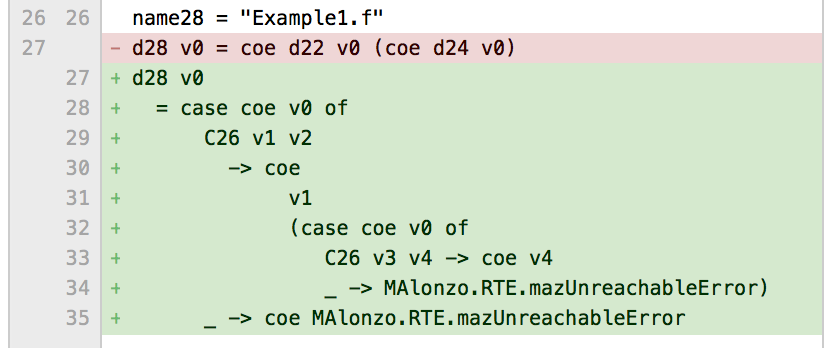
\includegraphics[width=0.5\textwidth]{Figures/Example1_inline}
    \caption{Unified difference of the \AgdaModule{Example1}~module compiled without and then with \texttt{-{}-inline-proj}.}
    \label{fig:Example1_inline}
\end{figure}

The compiled projection function \AgdaField{Pair.snd}, that is \lstinline{d18} in the Haskell code, is replaced with a Haskell expression that cases on the pair (\AgdaFunction{p} in Agda, \lstinline{d22} in Haskell) and returns the second field.

\begin{figure}[h!]
    \centering
    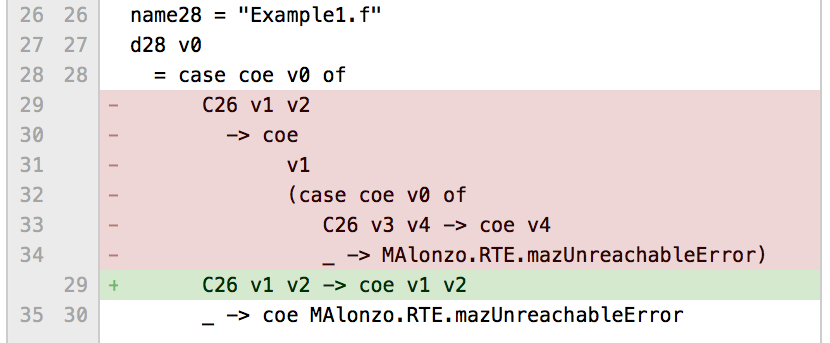
\includegraphics[width=0.5\textwidth]{Figures/Example1_squash}
    \caption{Unified difference of the \AgdaModule{Example1}~module compiled  with \texttt{-{}-inline-proj} and then also with \texttt{-{}-squash-cases}.}
    \label{fig:Example1_squash}
\end{figure}

We then compile the same file with both \texttt{-{}-inline-proj} and \texttt{-{}-squash-cases}, and the difference between only inlining and both inlining and squashing can be seen in Figure~\ref{fig:Example1_squash}.

\begin{figure}[h!]
    \centering
    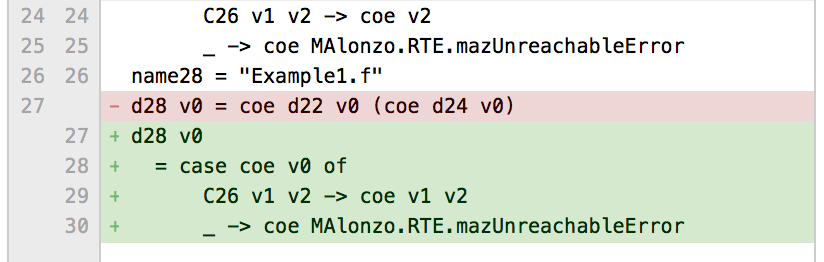
\includegraphics[width=0.5\textwidth]{Figures/Example1_inline_squash}
    \caption{Unified difference of the \AgdaModule{Example1}~module compiled without either optimisation, then with both \texttt{-{}-inline-proj} and \texttt{-{}-squash-cases}.}
    \label{fig:Example1_inline_squash}
\end{figure}

Figure~\ref{fig:Example1_inline_squash} shows the overall unified diff from neither optimisation to both.

\newpage

\section{RATH-Agda Main}
\label{sec:app_one}

RATH-Agda is a basic category and allegory theory library developed by Kahl, et al.\cite{kahl2017} It includes theories relating to semigroupoids, division allegories, typed Kleene algebras and monoidal categories, among other topics.\cite{kahl2017} The RATH-Agda repository also provides a set of test cases in a \AgdaModule{Main} module, which can be used to test a variety of typical uses of the library's functions.

\subsection{Before}

In profiling the runtime of this \AgdaModule{Main} module, we found that an inordinate amount of time was spent on evaluating simple record projections. The first few lines of the profiling report in Figure~\ref{fig:main_prof} indicate that the greatest cost centres in terms of time are the two simple record projections for the $\Sigma$ data type, with a combined 17.6\% of execution time spent evaluating them.

Because enabling profiling does have an affect on execution, we also re-compiled the module without profiling and ran it six times, measuring execution time with the Unix \texttt{time} command, to determing its average runtime as 1.60 seconds.

\begin{figure}
\begin{verbatim}
        Time and Allocation Profiling Report  (Final)

           Main +RTS -S -H7G -M7G -A128M -p -RTS

        total time  =        6.75 secs   (6755 ticks @ 1000 us, 1 processor)
        total alloc = 1,300,428,688 bytes  (excludes profiling overheads)

COST CENTRE                                                 %time %alloc

Data.Product.Σ.proj₂                                         10.4    0.0
Data.Product.Σ.proj₁                                          7.2    0.0
Categoric.KleeneCategory.DirectSum.SumStar.Square.E⋆′         4.9    7.0
Data.SUList.ListSetMap.RawLSM.RawLSM3.RawLSM3-comp.comp       4.1   10.4
Data.SUList.ListSetMap.RawLSM.RawLSM3.RawLSM3-comp.comp₀      3.9    3.7
...
\end{verbatim}
\caption{Profiling report for RATH-Agda's \AgdaModule{Main} module, compiled without projection inlining.}
\label{fig:main_prof}
\end{figure}


\subsection{After}

By compiling \AgdaModule{Main} with our new option, \texttt{-{}-inline-proj}, enabled, we reduced total runtime and memory allocation, as can be seen by comparing Figure~\ref{fig:main_inline_prof} and Figure~\ref{fig:main_prof}.

We again re-compiled the module without profiling and ran it six times, measuring execution time with the Unix \texttt{time} command, to determing its average runtime with projections inlined as 1.44 seconds. We therefore produced a speedup of 1.11$\times$.

\edcomm{NP}{Make a table out of those 6 trials}

\begin{figure}[h!]
\begin{verbatim}
        Time and Allocation Profiling Report  (Final)

           Main +RTS -S -H7G -M7G -A128M -p -RTS

        total time  =        5.26 secs   (5261 ticks @ 1000 us, 1 processor)
        total alloc = 1,299,709,408 bytes  (excludes profiling overheads)

COST CENTRE                                                 %time %alloc

Data.SUList.ListSetMap.FinRel.Utils.FinId                     6.2    8.6
Data.SUList.ListSetMap.RawLSM.RawLSM3.MapImage.mapImage₀      5.6    5.5
Data.SUList.ListSetMap.RawLSM.RawLSM3.RawLSM3-comp.comp       4.9    8.8
Categoric.KleeneCategory.DirectSum.SumStar.Square.E⋆′         4.7    6.6
Data.SUList.ListSetMap.Semigroupoid.LSMJoinOp.\               3.8    8.3
...
\end{verbatim}
\caption{Profiling report for RATH-Agda's \AgdaModule{Main}~module, compiled with projection inlining enabled.}
\label{fig:main_inline_prof}
\end{figure}


\section{Triangle Module}

\edcomm{NP}{Explain what this module does}

When we compile this module once without \texttt{-{}-ghc-generate-pattern-let} on, and once again with \texttt{-{}-ghc-generate-pattern-let} enabled, a unified diff of the two generated Haskell files gives us what is shown in Figure~\ref{fig:Triangle_genplet}. Both times, the module was compiled with \texttt{-{}-inline-proj}.

\begin{figure}[h]
    \centering
    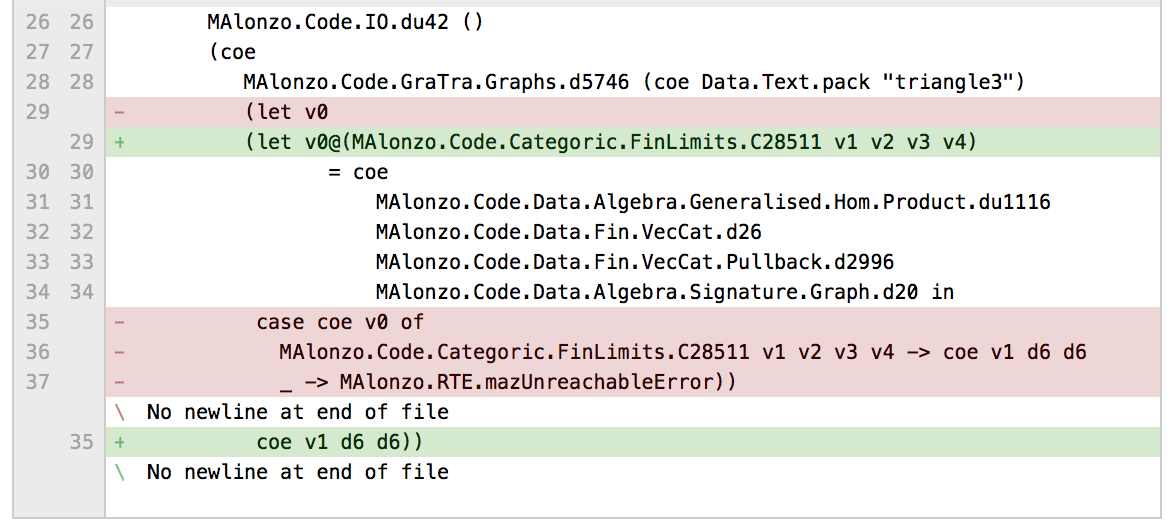
\includegraphics[width=0.5\textwidth]{Figures/Triangle_genplet}
    \caption{Unified difference of the \AgdaModule{Triangle3sPB}~module compiled without and then with \texttt{-{}-ghc-generate-pattern-let}.}
    \label{fig:Triangle_genplet}
\end{figure}

As is shown by this difference, the case analysis on \lstinline{v0} is no longer required and instead the constructor paramters are immediately bound in the enclosing \lstinline{let} expression.

\edcomm{NP}{Time and space results}


% Discussion and Conclusion
\setcounter{figure}{0}
\setcounter{equation}{0}
\setcounter{table}{0}
\chapter{Conclusion}
\label{cha:conclusion}

In this chapter, we discuss various aspects of our optimisations in summary. In Section~\ref{sec:assessment_of_the_contributions}, we assess the strengths and weaknesses of the main contributions. In Section~\ref{sec:future_work}, we discuss future work that could follow this project. Finally, in Section~\ref{sec:closing_remarks}, we draw conclusions from the thesis and give some closing remarks.

\section{Assessment of the Contributions}
\label{sec:assessment_of_the_contributions}

\subsection{Strengths of the Contributions}
\label{sub:strengths_of_the_contributions}

The contributions described herein have a number of strengths that will serve the Agda development community.

Primarily, as shown by the results of the applications of our optimisations in Section~\ref{cha:application_of_main}, our optimisations will reduce the runtime execution and heap allocation requirements of many Agda programs with a negligible impact on compile time, and do not show adverse effects in any of the tests we have performed.

Secondarily, this thesis may also serve as a detailed documentation of the portions of the Agda compiler and GHC backend that are necessary to understand for incorporating future optimising transformations. We hope that future contributors to Agda will find this presentation of our study of the Agda compiler useful in implementing their own desired optimisations.

\subsection{Weaknesses of the Contributions}
\label{sub:weaknesses_of_the_contributions}

Although the net effect of our optimisations is a positive one, there are still a number of weaknesses that warrant consideration.

A clear weakness of our case squashing optimisation is its isolated implementation. Because it was developed as an independent transformation, it requires an additional traversal of the treeless terms to execute. Further, some of the logic built to deal with the handling of de Bruijn indices would have been avoidable had it been built as part of an existing set of optimisations that had similar optimisation helper functions already developed. As presented in Subsection~\ref{sub:alternate_case_squash}, an independent version of case squashing has since been developed and introduced into the Agda compiler, as part of the \lstinline{Agda.Compiler.Treeless.Simplify} module, which addresses both of these weaknesses.

Both the projection inlining and case squashing optimisations make use of accumulated environment parameters, which can be handled more modularly and appropriately using monads. This potential for code refactoring is discussed further in Section~\ref{sec:future_work}.

\section{Future Work}
\label{sec:future_work}

In our implementations of projection inlining and case squashing, it was noted that environments of relevant information were carried through graph traversal. For projection inlining, this was an environment of previously inlined projections is maintained to avoid looping on recursive inlining calls. For case squashing, this was an environment of previously met cases expressions. These environments are currently maintained as a list objects, passed from function call to function call. For modularity and maintainability of the code, these environments would be better refactored into reader monad transformers, which would allow an inherited environment to be bound to the function results and passed through to subcomputations via the given monad.

Further testing of the projection inlining optimisation on a greater variety of Agda codebases is also a necessary next step before it can be safely integrated with a stable release branch of the compiler.

\section{Closing Remarks}
\label{sec:closing_remarks}

We have implemented, tested, and profiled a series of optimisations to the Agda compiler which improve execution time and reduce memory usage for many of the Agda programs tested, and have no negative performance effects in any of our tests. Our optimisations have a negligible impact on compile time, and serve previously unmet needs of our team as well as many other Agda developers.


% Appendices
\setcounter{figure}{0}
\setcounter{equation}{0}
\setcounter{table}{0}
\appendix
\chapter{Simplify.hs (abridged)}
\label{app:simplify}

\lstinputlisting[style=appendixhaskell]{Figures/Haskell/Simplify.hs}

\chapter{ToTreeless.hs (abridged)}
\label{app:to_treeless}

\lstinputlisting[style=blockhaskell]{Figures/Haskell/ToTreeless.hs}

\chapter{Case Squash.hs}
\label{app:case_squash}

\lstinputlisting[style=appendixhaskell]{Figures/Haskell/CaseSquash.hs}

\chapter{Compiler.hs (abridged)}
\label{app:compiler}

\lstinputlisting[style=appendixhaskell]{Figures/Haskell/Compiler.hs}


% Bibliography
% TODO
\edcomm{WK}{Look into natbib --- read the manual first.
(locate natbib | grep pdf)
The RATH-Agda documents (RATH-Agda/trunk/*.ltx) (at least mostly) use it, too, so you can check there. There is also RATH-Agda/trunk/bib/ref.bib ...}

\bibliographystyle{alpha}
\addcontentsline{toc}{chapter}{Bibliography}
\bibliography{Bibliography/ref}

% Index
\newpage
\addcontentsline{toc}{chapter}{Index}
\printindex

\end{document}
%________________________________________________________________________
